\documentclass[main.tex]{subfiles}
% 标架与参考系
\begin{document}
\subsection{新古典时空}
在经典力学中,我们认为物理事件的发生是不依赖于人的观察与否或观察方式的客观事实。我们希望,同一件物理事件,经不同的观察者观察后作出的报告,能通过一套互译系统而统一成一个结论;不同观察者通过对实验观测的总结归纳,可以达成一个不依赖具体观察者的情境和观察方式的、关于大自然规律性的共识。这种情况称为物理客观性\cite{Reiss2020}。

\begin{figure}[h]
    \centering
    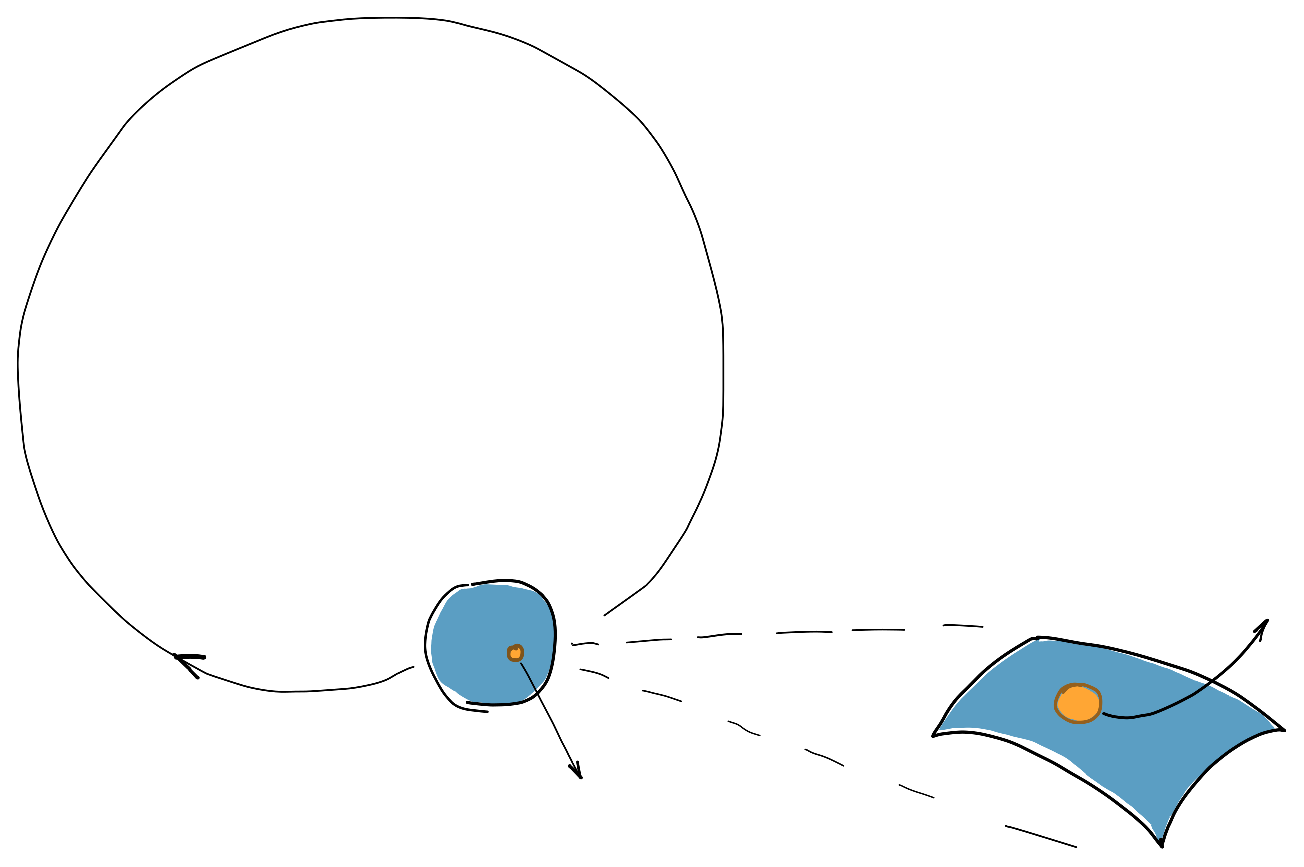
\includegraphics[width=0.5\textwidth]{images/III.1.1.eps}
    \caption{非惯性系下的运动规律。}
    \label{fig:III.1.1}
\end{figure}

\begin{example}[“我们” vs “球上的人”]
在一个相对我们作匀速(低速)圆周运动的球上站着的人(他看不到我们,但能与我们通讯交流),通过抓稳该球保持与球相对静止。他以球作参照物,研究球上的物体的运动,会得出:保持物体的静止需要一个方向恒定的力,因为球上的物体都需要绑在球上才能保持相对于球静止,他通过弹簧秤可以测量出这一力的大小,进一步发现保持物体静止的力与该物体的质量成正比。如果把某物体松绑,使其不受任何力,物体会开始作一个曲线运动。我们则能不通过测量力就看到球和球上的物体的圆周运动,在我们眼中它们的运动状态是一直在改变中的,而不是静止的;给物体松绑后,物体以松绑时的速度作为初速度作匀速直线运动(如图\ref{fig:III.1.1}所示)。故我们的观察符合“物体在没有外力作用的情况静止或作匀速直线运动”的论断。如果球的匀速圆周运动的角速度发生变化,我们仍然能不通过力的测量而看到这一点,但球上的人只会发现,保持球上物体静止所需的力的大小在莫名其妙地变化。如果他在球上设置一个单摆,他将发现单摆的摆动方向在随时间变化,而我们认为这个单摆的摆动方向没有变化。总而言之,我们认为牛顿力学定律符合实际,但球上的人将不会同意。但他和我们通过通讯至少能确认双方所观察的现象是同一个物理现象,按照物理客观性原则理应受同一套自然定律统治。摆在他和我们面前的任务只是如何构造一套理论统一地描述好这一自然定律。
\end{example}

在经典力学中,一个物理事件的发生,同时具有“发生的位置”和“发生的时刻”这两个属性。一名观察者使用时钟测量两个物理事件发生的时间间隔,使用直尺来测量两个物理事件发生位置之间的距离。其中距离的测量总是针对同时刻发生的两个事件。

\begin{figure}[h]
\centering
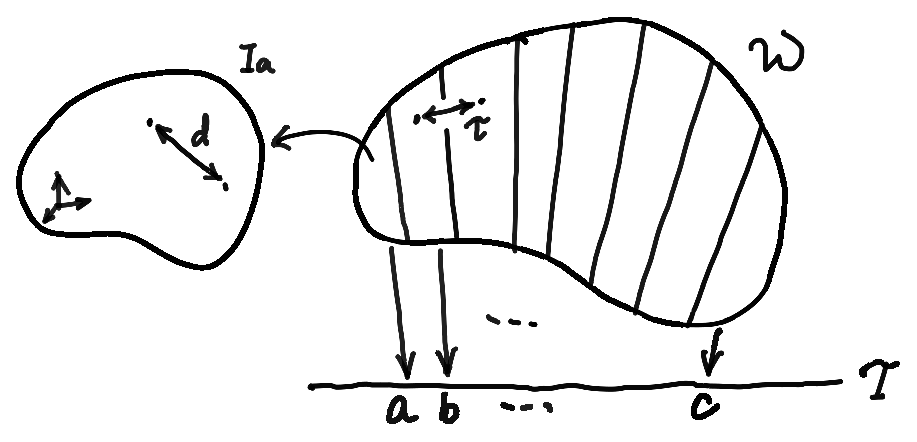
\includegraphics[width=0.5\textwidth]{images/III.1.2.eps}
\caption{事件世界与同时等价类示意图}
\label{fig:III.1.2}
\end{figure}

引入事件世界$\mathcal{W}$。

\begin{definition}[事件世界、时间]
$\mathcal{W}$是一个非空集,其元素$w\in\mathcal{W}$称为一个事件。我们给予$\mathcal{W}$一个函数$\tau:\mathcal{W}^2\rightarrow\mathbb{R}$,满足:
\begin{itemize}
    \item $\forall a,b\in\mathcal{W}:\tau\left(a,b\right)=-\tau\left(b,a\right)$
    \item $\forall a,b,c\in\mathcal{W}:\tau\left(a,b\right)+\tau\left(b,c\right)=\tau\left(a,c\right)$
    \item $\forall a\in\mathcal{W},t\in\mathbb{R},\exists b\in\mathcal{W}:\tau\left(a,b\right)=t$
\end{itemize}
我们称$\tau$为(两事件的)时间间隔或时长。我们还能称
\begin{itemize}
    \item 事件$a$早于事件$b$当且仅当$\tau\left(a,b\right)>0$
    \item 事件$a$晚于事件$b$当且仅当$\tau\left(a,b\right)<0$
    \item 事件$a$与$b$同时当且仅当$\tau\left(a,b\right)=0$
\end{itemize}
上面的第三条给出了两事件的同时性。易验同时性是一个等价关系,即$S=\left\{\left(a,b\right)|\tau\left(a,b\right)=0\right\}$满足自反性、传递性、对称性。这一等价关系将事件世界$\mathcal{W}$划分为等价类,即:
\[\mathcal{W}=\bigcup_{a\in\mathcal{T}}I_a,I_a=\left\{x\in\mathcal{W}|\tau\left(a,x\right)=0\right\}\]
其中等价类$I_a$称为时刻$a$对应的同时等价类,它是所有与事件$a$同时的事件的子集,而$a$在此变成了时刻的标记,集合$\mathcal{T}$称为时间,是所有(不同)时刻的集合(如图\ref{fig:III.1.2}所示)。

我们还给予事件世界$\mathcal{W}$以一个度量$d:I_a\times I_a\rightarrow\mathbb{R},a\in\mathcal{T}$,称两事件间的“距离”,它还要满足:
\begin{itemize}
    \item $d$是$I_a$上的一个欧几里德度量,故$I_a$是一个欧几里德空间,带有一个平移空间$\mathcal{V}_a$。
    \item $\forall a\in\mathcal{T}:\mathrm{dim}\mathcal{V}_a=3$
\end{itemize}
注意到,这一度量只能作用在同时发生的两个事件上的(如图\ref{fig:III.1.2}所示)。
\end{definition}

结合度量$\tau$的定义,$\left(\mathcal{T},\left|\tau\right|\right)$形成一个度量空间。在此度量空间上的等距变换拥有之前介绍过的一切性质。值得注意的是,由$\tau$的定义,可知$\mathcal{T}$的平移空间是一维的、完备的。我们可直接使用实数集$\mathbb{R}$作为其平移空间。选定某时刻$t_0\in\mathcal{T}$作为原点,$\mathbb{R}$的正或负作为时间流逝的方向以及单位时长(相当于在作为向量空间的$\mathbb{R}$中选择了一个规范正交基),则由等距变换的表示定理(定理\ref{thm:II.11.4})对任一$\mathcal{T}$上的等距变换$i:\mathcal{T}\rightarrow\mathcal{T}$有$i\left(t\right)=i\left(t_0\right)+ Q\left(t-t_0\right)$。其中$Q=\pm 1$时间正方向的选择。由于我们很少遇到两个观察者记录时间的方式是反号的情况,因此常常只讨论(默认)$Q=1$,即
\[
i\left(t\right)=i\left(t_0\right)+\left(t-t_0\right)
\]

\begin{figure}[h]
    \centering
    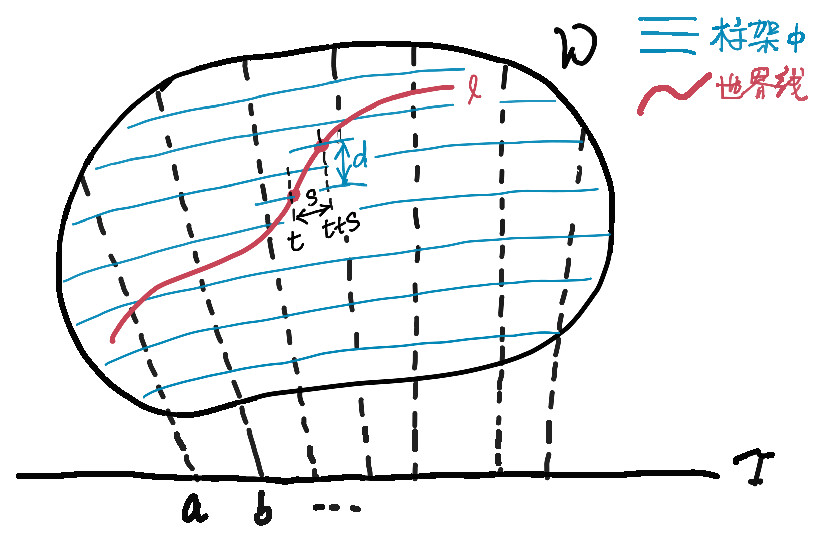
\includegraphics[width=0.5\textwidth]{images/III.1.3.eps}
    \caption{世界线及事件世界的标架示意图}
    \label{fig:III.1.3}
\end{figure}

\subsection{世界线与标架}
引入世界线的概念。

\begin{definition}[世界线]
世界线是由时间$\mathcal{T}$到事件世界$\mathcal{W}$的单射$l:\mathcal{T}\rightarrow\mathcal{W}$。
\end{definition}

一条世界线$l\left(t\right),t\in\mathcal{T}$的任意两个值都是属于不同时刻的事件(如图\ref{fig:III.1.3}所示)。一条世界线是某质点运动轨迹的客观存在(即不依赖人的观察与否与观察方式的独立概念)。

依赖世界线的概念,我们可以引入“事件世界的标架”的概念。

\begin{definition}[事件世界的标架]
事件世界的标架$\phi$是一组“平行”的世界线$\left\{l,\cdots\right\}$(如图\ref{fig:III.1.3}所示),其元素$l\in\phi$称为标架线。“平行”的意思是对任意两时刻$t_1,t_2\in\mathcal{T}$两条世界线$l_1,l_2\in\phi$有$d\left(l_1\left(t_1\right),l_2\left(t_!\right)\right)=d\left(l_1\left(t_2\right),l_2\left(t_2\right)\right)$。一个标架的所有标架线还要覆盖整个事件世界的所有事件,即
\[\bigcup_{l_i\in\phi}\mathrm{ran}l_i=\mathcal{W}\]
使得没有一个事件是不属于任何标架线的。映射$l_\phi:\mathcal{W}\rightarrow\phi,l_\phi\left(a\right)=\left\{l|l\in\phi,a\in\mathrm{ran}l\right\}\forall a\in\mathcal{W}$是为任一事件找到其所属的标架线的映射。由标架线“平行”的性质易验$\left\{l|l\in\phi,a\in\mathrm{ran}l\right\}$有且只有一个元素,即任一事件$a\in\mathcal{W}$对应且只对应一条标架线,且有$d\left(l_\phi\left(a\right)\left(t\right),l_\phi\left(b\right)\left(t\right)\right)=\text{常数}\forall a,b\in\mathcal{W},t\in\mathcal{T}$,故可由此定义“标架线之间的距离”:
\[d\left(l_\phi\left(a\right),l_\phi\left(b\right)\right)=d\left(l_\phi\left(a\right)\left(t\right),l_\phi\left(b\right)\left(t\right)\right),t\in\mathcal{T}\]
映射$l_\phi$还具有性质$l_\phi\left(l_\phi\left(a\right)\left(t\right)\right)=l_\phi\left(a\right)\forall t\in\mathcal{T},a\in\mathcal{W}$。
\end{definition}

总结标架的特点:
\begin{itemize}
    \item 由于标架线是世界线,故它贯穿了不同时刻;
    \item 任一事件必属于某标架线;
    \item 我们可以谈论两条标架线之间的距离;
\end{itemize}
可知,标架的重要意义是使得我们可以讨论不同时刻的任意两个事件$a\in I_{t_1},b\in I_{t_2},t_1,t_2\in\mathcal{T}$之间的距离,选定标架$\phi$,$a$与$b$的距离就是$d\left(l_\phi\left(a\right),l_\phi\left(b\right)\right)$。

例如,既然一条世界线所代表的某质点的运动过程,那么我们直觉上会想要通过形如下式的导数来定义“速度”:
\[
\lim_{s\to 0}\frac{l\left(t+s\right)-\l\left(t\right)}{s}\]
但是,上式的分子中相减的两个事件是属于不同时刻的同时等价类的($l\left(t+s\right)\in I_{t+s},l\left(t\right)\in I_t,t+s,t\in\mathcal{T}$,如图\ref{fig:III.1.3}所示),因此这个减法的意义是没有定义的。通过事件世界的标架$\phi$,我们可以解决这个问题,从而定义速度$\mathbf{v}:\mathcal{T}\rightarrow\mathcal{V}_\phi$:
\[\mathbf{v}\left(t_0\right)=\lim_{t\to t_0}\frac{l_\phi\left(l\left(t\right)\right)-l_\phi\left(l\left(t_0\right)\right)}{t}\]
上式的速度定义利用了$\left(\phi,d\right)$是一个欧几里德度量空间的事实,分子中相减的两个元素是标架$\phi$中的两条世界线。它们的差对应$\mathcal{V}_\phi$中的一个平移向量。故速度是一个向量且依赖标架$\phi$的选择。注意到,在速度的定义过程中我们默认了一切需要的连续性。加速度也可以类似地被定义,且由于相同的原因加速度也依赖标架$\phi$的选择。我们称标架$\phi$的选择是主观的。依赖$\phi$定义的概念都是不具有物理客观性的(除非增加某些限定条件)。

考虑任一时刻$t\in\mathcal{T}$对应的同时等价类$I_t$。选定某标架$\phi$后,易证$I_t$中的任意两个不同的事件不可能属于同一条标架线,反之亦然。故映射$l_\phi$限定在某同时等价类$I_t$上是双射。同为欧几里德度量空间的$\left(I_t,d\right)$和$\left(\phi,d\right)$,它们对应的平移空间$\mathcal{V}_t,\mathcal{V}_\phi$同构,故$\mathrm{dim}\mathcal{V}_\phi=\mathrm{dim}\mathcal{V}_t=3$。对于一系列不同时刻的同时等价类$I_{t_1},I_{t_2},\cdots$,它们各自都对应一个平移空间$\mathcal{V}_{t_1},\mathcal{V}_{t_2},\cdots$,且$\mathrm{dim}\mathcal{V}_{t_1}=\mathrm{dim}\mathcal{V}_{t_2}=\cdots=\mathrm{dim}\mathcal{V}_\phi$,即标架的平移空间$\mathcal{V}_\phi$与每个时刻的同时等价类的平移空间都同构。我们于是可以统一采用$\mathcal{V}_\phi$作为每个时刻的同时类的平移空间,不同时刻下的事件的位置,我们都用统一的一套平移向量描述。

\begin{figure}[h]
\centering
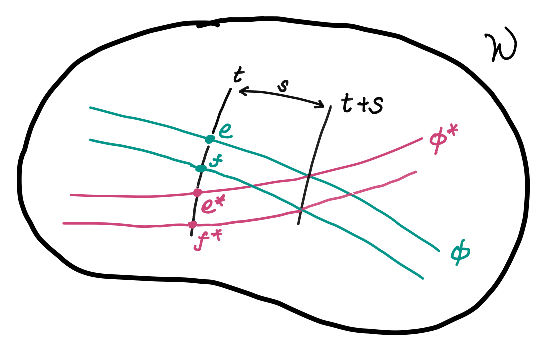
\includegraphics[width=0.5\textwidth]{images/III.1.4.eps}
\caption{事件世界的标架变换示意图}
\label{fig:III.1.4}
\end{figure}

考虑事件世界$\mathcal{W}$中的两组不同的标架$\phi,\phi^*$。事件$e\in I_t$的时刻是$t\in\mathcal{T}$,其所属的$\phi$中的标架线是$l_\phi\left(e\right)$。考虑距时刻$t$间隔为$s\in\mathbb{R}$的另一时刻$t+s$,该时刻在标架线$l_\phi\left(e\right)$上的事件是$l_\phi\left(e\right)\left(t+s\right)$。该事件在标架$\phi^*$中所属的标架线是$l_{\phi^*}\left(l_\phi\left(e\right)\left(t+s\right)\right)$,在该标架线上$t$时刻的事件是$l_{\phi^*}\left(l_\phi\left(e\right)\left(t+s\right)\right)\left(t\right)\in I_t$(如图\ref{fig:III.1.4}所示)。令
\[e^*=l_{\phi^*}\left(l_\phi\left(e\right)\left(t+s\right)\right)\left(t\right)\]
则有$l_{\phi^*}\left(e^*\right)=l_{\phi^*}\left(l_\phi\left(e\right)\left(t+s\right)\right)$。设$e,f\in I_t,e\neq f$,则有
\[
    d\left(e^*,f^*\right)=d\left(l_{\phi^*}\left(l_\phi\left(e\right)\left(t+s\right)\right),l_{\phi^*}\left(l_\phi\left(f\right)\left(t+s\right)\right)\right)
\]
由恒等关系$l_{\phi^*}\left(l_\phi\left(e\right)\left(t\right)\right)\left(t\right)=l_\phi\left(e\right)\left(t\right)\forall e\in\mathcal{W},t\in\mathcal{T}$,上式$\Leftrightarrow$
\begin{align*}
    d\left(l_\phi\left(e\right)\left(t+s\right),l_\phi\left(f\right)\left(t+s\right)\right)&=d\left(l_\phi\left(e\right)\left(t\right),l_\phi\left(f\right)\left(t\right)\right)\\
    &=d\left(e,f\right)
\end{align*}
因此,对任意$e,f\in\mathcal{W}$,$d\left(l_\phi\left(e\right),l_\phi\left(f\right)\right)=d\left(l_{\phi^*}\left(e^*\right),l_{\phi^*}\left(f^*\right)\right)$,即由$\phi$到$\phi^*$存在一个等距映射。由等距映射的表示定理,选定$\phi$中的一标架线$l_0$,则$l*\left(s\right)=l_0^*\left(s\right)+\mathbf{Q}\left(s\right)\left(l-l_0\right),l\in\phi,l^*\in\phi^*$,其中$l_0^*=l_{\phi^*}\left(l_\phi\left(l_0\right)\left(t+s\right)\right)$。我们称这一变换为一个标架变换。一个标架变换不仅包括了上述的标架线之间的等距变换,还隐含包括了一个$\mathcal{T}$的等距变换(即选定了参考时刻$t$并将任一时刻表示为$t+s$)。

上述关于事件世界、世界线、标架的概念构建方式,代表着我们观测物理事件的实际方式。一位观察者总是把所观察到的空间理解为3维欧几里德空间。他用一把直尺测量同一时刻两物理事件的距离,用一个时钟测量两物理事件的时间间隔。在某时刻下,选定空间中一点作为参照点和过该点三条两两不共线的射线方向作为参考方向——即坐标系,则空间中任一点都能通过从参照点到该点的方向和距离(即平移向量)的得到唯一标示。选择某一时刻作为参考时刻,则任一时刻都可通过与参考时刻之间的时长得到标示。坐标系与这一参考时刻的选择,统称参考系。一个观察者在某时刻选择的坐标系会在其他时刻延用;这相当于选定了一个标架$\phi$并实际统一采用$\mathcal{V}_\phi$中的向量作来任一时刻下的平移向量。

两名观察者,观察同一事件,他们首先要相互对表,即在某时刻两人用各自的钟表同时开始计时,经过相同的时长后,两人得出双方钟表读数的差别。这是在时间$\mathcal{T}$内的一个等距变换。对完表之后,两人选取同一时刻作为参考时刻,对同一物理事件进行观察。由于两人选取的坐标系可能是不同的,因此两人还需要在同一时刻确认对方所找的坐标系;然后,其中一人除了要观察所关注的物理事件在自己所选择的坐标系下随时间的变化之外,还要观察对方选择的坐标系在自己选择的坐标系下随时间的变化,才能知道任一时刻,同一物理事件在对方坐标系下的表示。每个时刻,两个坐标系的之间的关系都可能是不同的,故它们之间的转换是依赖时刻的等距变换。

\subsection{标架的简化定义}
一名观察者如果选定了参考时刻$t_0$和标架$\phi$,则任一时刻都能对应$\mathbb{R}$中的一个实数。选定$\mathcal{V}_\phi$中的一向量$\mathbf{\hat{o}}$和一组基$\left\{\mathbf{\hat{e}}_i\right\}$,则任一时刻发生的物理事件的位置都能对应到$\mathbb{R}^3$中的一个坐标。为了实用性,我们可以把标架重新定义为一名观测者从$\mathcal{W}$直接到$\mathbb{R}^{3+1}$的对应过程,即$\phi:\mathcal{W}\rightarrow\mathbb{R}^{3+1}$。这时,标架$\phi$实际包括了一个观察者对$t_0$、$\mathbf{\hat{o}}$和$\left\{\mathbf{\hat{e}}_i\right\}$的主观选择。标架变换仍然包括时间和空间的两个等距变换,与原意义的标架变换是相同。

具体地,任一事件$w\in\mathcal{W}$经标架$\phi$映射为$\left(\mathbf{x},t\right),\mathbf{x}\in\mathbb{R}^3,t\in\mathbb{R}$,经标架$\phi^*$映射为$\left(\mathbf{x}^*,t^*\right),\mathbf{x}^*\in\mathbb{R}^3,t^*\in\mathbb{R}$。我们认为$\phi,\phi^*$是可逆的,故有$\left(\mathbf{x}^*,t^*\right)=\phi^*\circ\phi^{-1}\left(\mathbf{x},t\right)$。若$w$的时刻是$a\in\mathcal{T}$,标架$\phi$选择的时间原点是$t_0$,标架$\phi^*$选择的时间原点是$t_0^*$,则时间的度量空间上的一个等距变换$g:\mathcal{T}\rightarrow\mathcal{T}$可表示为
\[t^*=g\left(t\right)=t_0^*+\tau\left(t-t_0\right),t_0^*=g\left(t_0\right)\]
若标架$\phi$和$\phi^*$选择的空间原点分别是$\mathbf{x}_0,\mathbf{x}_0^*$,则在时刻$a$由标架$\phi$到标架$\phi^*$的变换是一个等距变换$i_a:\mathbb{R}^3\rightarrow\mathbb{R}^3$,
\[\mathbf{x}^*=i_a\left(\mathbf{x}\right)=i_a\left(\mathbf{x}_0\right)+\mathbf{Q}_a\left(\mathbf{x}-\mathbf{x}_0\right),\mathbf{x}_0^*=i_a\left(\mathbf{x}_0\right)\]
所以,由$\phi$到$\phi^*$的标架变换包含一个时间的等距变换$g$和一个空间的等距变换$i_a$,其中$a$是事件的时刻。

\subsection{场函数的标架不变性}
设$\left(\mathbf{x}^*,t^*\right),\left(\mathbf{y}^*,t^*\right)$与$\left(\mathbf{x},t\right),\left(\mathbf{y},t\right)$是同一事件在标架$\phi,\phi^*$下的坐标和时标,则有$\mathbf{x}^*=\mathbf{x}_0^*\left(t\right)+\mathbf{Q}\left(t\right)\left[\mathbf{x}-\mathbf{x}_0\right],\mathbf{y}^*=\mathbf{x}_0^*+\mathbf{Q}\left(t\right)\left[\mathbf{y}-\mathbf{x}_0\right]$。两式相减得
\[\mathbf{y}^*-\mathbf{x}^*=\mathbf{Q}\left(t\right)\left(\mathbf{y}-\mathbf{x}\right)\]
我们知道$\left(\mathbf{x}^*,t^*\right)$与$\left(\mathbf{x},t\right)$对应是同一事件;同样地$\left(\mathbf{y}^*,t^*\right)$与$\left(\mathbf{y},t\right)$也对应同一事件。故上式是同一向量在一个标架变换下的关系式。设$\mathbf{A}\in\mathcal{L}\left(\mathbb{R}^3\right)$是$\mathbb{R}^3$上的任一张量,$\mathbf{v}=\mathbf{y}-\mathbf{x},\mathbf{v}^*=\mathbf{y}^*-\mathbf{x}^*$。则有
\[\mathbf{A}^*\mathbf{v}^*\equiv\left(\mathbf{Av}\right)^*=\mathbf{Q}\left(t\right)\mathbf{AQ}^\intercal\left(t\right)\mathbf{v}^*
\]
其中我们利用了$\mathbf{Q}^{-1}=\mathbf{Q}^\intercal$。上式是同一张量在一个标架变换下的关系式。

设在标架$\phi,\phi^*$下,标量场函数$h=h\left(\mathbf{x},t\right),h^*=h^*\left(\mathbf{x}^*,t^*\right)$,向量场函数$\mathbf{v}=\mathbf{v}\left(\mathbf{x},t\right),\mathbf{v}^*=\mathbf{v}^*\left(\mathbf{x}^*,t^*\right)$,张量场函数$\mathbf{A}=\mathbf{A}\left(\mathbf{x},t\right),\mathbf{A}^*=\mathbf{A}^*\left(\mathbf{x}^*,t^*\right)$,则
\begin{itemize}
    \item 当且仅当$h^*\left(\mathbf{x}^*,t^*\right)=h\left(\mathbf{x},t\right)$时称$h$——
    \item 当且仅当$\mathbf{v}^*\left(\mathbf{x}^*,t^*\right)=\mathbf{Q}\left(t\right)\mathbf{v}\left(\mathbf{x},t\right)$时称$\mathbf{v}$——
    \item 当且仅当$\mathbf{A}^*\left(\mathbf{x}^*,t^*\right)=\mathbf{Q}\left(t\right)\mathbf{A}\left(\mathbf{x},t\right)\mathbf{Q}^\intercal\left(t\right)$时称$\mathbf{A}$——
\end{itemize}
具有标架不变性。
\end{document}